\documentclass[lettersize,journal]{IEEEtran}
\usepackage{amsmath,amsfonts}
\usepackage{algorithmic}
\usepackage{algorithm}
\usepackage{array}
\usepackage[caption=false,font=normalsize,labelfont=sf,textfont=sf]{subfig}
\usepackage{textcomp}
\usepackage{stfloats}
\usepackage{url}
\usepackage{hyperref}
\usepackage{verbatim}
\usepackage{graphicx}
\usepackage{cite}
\hyphenation{op-tical net-works semi-conduc-tor IEEE-Xplore}
% updated with editorial comments 8/9/2021
\usepackage{tikz}
\usepackage{svg}
\usepackage{amsfonts}
\usepackage{amsmath}
\usepackage{bbm}
\usepackage{mathtools}
\usepackage{makecell}
\usepackage{multirow}
\usepackage[none]{hyphenat}
\sloppy

\usepackage{adjustbox}

\begin{document}
\title{Interpretable Anomaly Detection in the LHC Main Dipole Circuits with Non-Negative Matrix Factorization}

\author{Christoph Obermair, Andrea Apollonio, Zinour Charifoulline, Lukas Felsberger, Marvin Janitschke, Franz Pernkopf, Emmanuele Ravaioli, Arjan Verweij, Daniel Wollmann, and Mariusz Wozniak % <-this % stops a space
\thanks{Christoph Obermair is with CERN, CH, 1211 Meyrin, Switzerland, and also with Graz University of Technology, AT, 8010 Graz, Austria (e-mail: christoph.obermair@cern.ch).}% 
\thanks{Andrea Apollonio, Zinour Charifoulline, Lukas Felsberger, Emmanuele Ravaioli, Arjan Verweij, Daniel Wollmann, Mariusz Wozniak are with CERN, CH, 1211 Meyrin, Switzerland.}% 
\thanks{Marvin Janitschke is with CERN, CH, 1211 Meyrin, Switzerland, and also with the University of Rostock, DE, 18051 Rostock, Germany.}% 
\thanks{Franz Pernkopf is with Graz University of Technology, AT, 8010 Graz, Austria.}%
\thanks{The code for this project is publicly available at \url{https://github.com/cobermai/lhc_anomaly_detection}}%
}

% The paper headers
\markboth{IEEE TRANSACTIONS ON APPLIED SUPERCONDUCTIVITY, VOL. x, NO. x, x}%
{Shell \MakeLowercase{\textit{et al.}}: A Sample Article Using IEEEtran.cls for IEEE Journals}

%\IEEEpubid{0000--0000/00\$00.00~\copyright~2021 IEEE}
% Remember, if you use this you must call \IEEEpubidadjcol in the second
% column for its text to clear the IEEEpubid mark.

\maketitle

\begin{abstract}
CERN's Large Hadron Collider (LHC) with its eight superconducting main dipole circuits has been in operation for over a decade. 
During this time, relevant operational parameters of the circuits, including circuit current, voltages across magnets and their coils, and current to ground, have been recorded. 
These data allow for a comprehensive analysis of the circuit characteristics, the interaction between their components, and their variation over time. 
Such insights are essential to understand the state of health of the circuits and to detect and react to hardware fatigue and degradation at an early stage.

In this work, a systematic approach is presented to better understand the behavior of the main LHC dipole circuits following fast power aborts. 
Non-negative Matrix Factorization is used to model the recorded frequency spectra as common sub-spectra, by decomposing the recorded data as a linear combination of basis vectors, which are then related to hardware properties.
The loss in reconstructing the recorded frequency spectra allows to distinguish between normal and abnormal magnet behavior. 
In the case of abnormal behavior, the analysis of the sub-spectra properties enables to infer possible hardware issues. 
Following this approach, five dipole magnets with abnormal behavior were identified, of which one was confirmed to be damaged. As three of the other four identified magnets share similar sub-spectra characteristics, they are also treated as potentially critical. These results are essential for preparing targeted magnet measurements and may lead to preventive replacements.
\end{abstract}

\begin{IEEEkeywords}
Large Hadron Collider, Quench Protection, Non-negative Matrix Factorization, Machine Learning
\end{IEEEkeywords}

\section{Introduction}

\IEEEPARstart{T}{he} LHC is the world's largest and highest energy particle accelerator, relying on 1232 superconducting main dipole magnets to bend the high-energy particle beams along its circumference. These dipole magnets are powered through eight separate circuits of 154 magnets each.
To reach the nominal field of 8.0~T and a current of 11.85~kA, each magnet is cooled down to 1.9~K with superfluid helium. 
At this temperature, the magnet is superconducting.
A resistive transition in a superconductive magnet, also called quench, results in local heating in the superconducting cables and high voltage transients in the magnet, which can possibly damage the magnet if not appropriately managed.
%Therefore, a system of protection elements is in place to ensure a fast and safe extraction of the energy stored in the magnets in case of a quench or other powering failures in the circuits~\cite{Schultz2002}. 
In case of a quench or other powering failures in the circuits, therefore, a system of protection elements is in place to safely dissipate the energy in the quenched magnets and extract the remaining energy of the circuit~\cite{Schultz2002}.
This process is referred to as a Fast Power Abort~(FPA) event. To better understand the data recorded during a FPA event, the LHC main dipole circuits and their protection system are explained in more detail below.

% LHC circuit
Figure~\ref{circuit} shows a schematic view of a main dipole circuit with its 154 magnets, each represented by a magnet inductance~$L_\text{M}$~\cite{ravaioli2012}.
For this analysis, the magnets are counted along their physical position from the left to the right or clockwise along the electrical connection starting from the Power Converter~(PC). 
%The PC is located at the even access points.
In case the PC is switched off, the current~$I$ circulating in the circuit by-passes the PC via the Crowbar~(CB).
The Current Leads~(CL) indicate the transition between the cold superconducting part of the circuit and the warm, normal conductive part of the circuit.

\begin{figure}
    \centering
    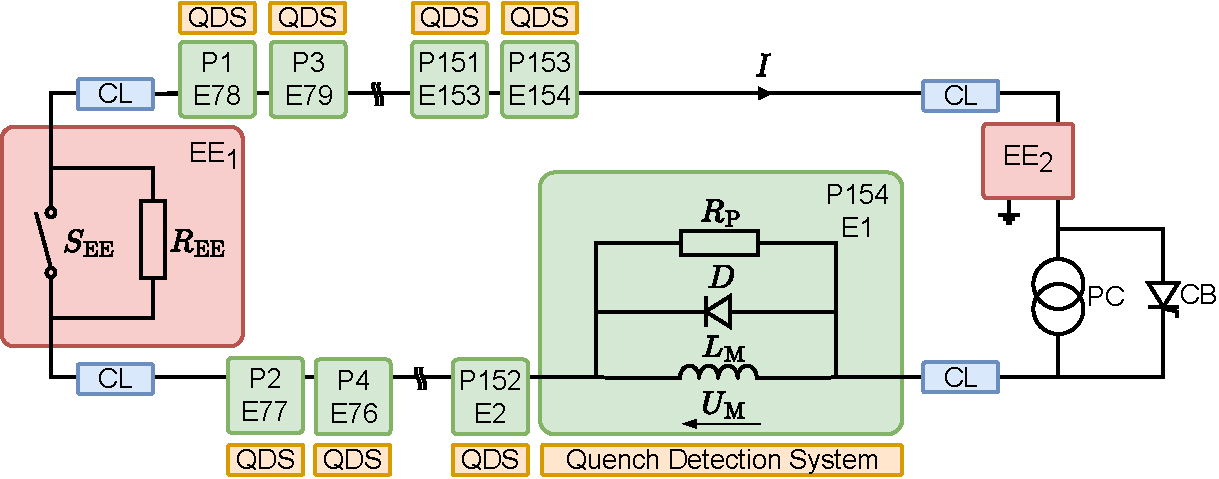
\includegraphics[width=0.49\textwidth]{figures/circuit_diagram.drawio.pdf}
    \caption{Schematic view of the main dipole circuit, including the Power Converter~(PC), the Crowbar~(CB) and the Current Leads~(CL). 
    The Quench Detection System~(QDS) triggers a Fast Power Abort~(FPA), which deactivates the PC and activates the energy extraction systems. Furthermore, it triggers the discharge of the quench heaters~(QH) in the respective magnet, if a quench is detected.
    The two Energy Extraction Systems EE\textsubscript{1} and EE\textsubscript{2} consist of a Switch~$S_\text{EE}$, and an Energy Extraction Resistance~$R_\text{EE}$. The circuit is grounded at the center of the resistor $R_\text{EE}$ in the EE\textsubscript{2} system. 
    The magnet with inductance $L_\text{M}$ and the by-pass Diode~$D$ with a Parallel Resistance~$R_\text{P}$ are in a liquid helium cryostat.
    Magnets are labeled by their Physical position~(P) from the left to the right. The Electrical positions~(E) are counted clockwise along the electrical connection starting from the PC. The numbering shown here is representing the circuits in sectors 12, 34, 56, and 78. In sectors 23, 45, 67, and 81 the electrical labels change, as the PC is on the left side of the circuit.
    }
    \label{circuit}
\end{figure}

% Quench protection   
The protection system includes a Quench Detection System~(QDS), which detects a quench and triggers the appropriate protection actions~\cite{Denz2006,Denz2009}.
Upon the detection of a quench in a dipole magnet, the PC is switched off and the Quench Heaters~(QH) of this magnet are activated.
QHs are resistive strips attached to the outer surface of each magnet coil~\cite{Rodriguez2000}.
They ensure protection by distributing the magnet's stored energy more uniformly over the quenched magnet windings~\cite{Sonnemann2001}. 
The by-pass Diode~$D$ diverts current from the quenched magnet.
This restricts the quenching magnet to only absorb its stored magnetic energy, not the energy of the entire circuit. The Parallel Resistance~$R_\text{P}$ installed across each magnet, smoothens transient voltages during this process~\cite{Bourgeois2001}. 
% Energy Extraction 
To avoid the circuit's energy to solely discharge in the diode of the quenched magnet, the Switches~$S_\text{EE}$ in both Energy Extraction~(EE) systems are sequentially activated~\cite{Dahlerup2002}.
They direct the circuit current towards the Resistances~$R_\text{EE}$, which extracts the circuit's energy within around 300~s. 
The voltages $U_\text{M}$ measured over the 154 magnets during a FPA event are shown in Fig.~\ref{timeseries}. 
These signals are voltage transients that contain information about the behavior of the electrical circuit and its components~\cite{2ravaioli2012}.

\begin{figure}
    \centering
    \includesvg[scale=0.85]{figures/u_mag.svg}
    \caption{Voltages $U_\text{M}$ across the 154 main dipole magnets of sector 78 following a quench in the magnet with the electrical position 141 on 31.03.2021 with its different phases: a) the FPA is triggered at 0~s, the QHs for magnet 141 are activated, and the PC is deactivated; b) after around 0.03~s the by-pass diode of the quenched magnet becomes conductive; c) the first Energy Extraction system EE\textsubscript{1} is activated about 0.1~s after the FPA trigger; d) the second Energy Extraction system EE\textsubscript{2} is activated approximately 0.5~s after the first one. 
    The blue curve shows the voltage across the quenched magnet, while the remaining curves represent the voltages across the other 153 magnets of the circuit. 
    The voltage signals of one of the analyzed plateaus are shown in the magnified view. }
    \label{timeseries}
\end{figure}

% Why we need to understand the circuit 
% In general, a quench is a routine occurrence, during training periods aimed at increasing the peak magnetic field in the superconducting magnets~\cite{verweij2008}.
% In addition, quenches also rarely occur during operation.
A quench is a routine occurrence, during training periods aimed at increasing the peak magnetic field in the superconducting magnets~\cite{verweij2008}, and rarely occurs during operation.
Once a quench emerges, it is frequently accompanied by secondary quenches. 
Secondary quenches result from electromagnetic perturbations milliseconds after the initial quench~\cite{ravaioli2012} or from temperature propagation in the helium tens of seconds later~\cite{Coull1996}.
Following a quench or a secondary quench, the magnet is exposed to local heating, high voltages, and thermal expansion, depending  on the circuit's energy level~\cite{siemko_magnet_2023}.
The magnets are designed with additional margins for this case, yet undetected defects may reveal themselves.
Certain hardware failures in the superconducting circuit during operation can notably impact the availability of the LHC, potentially resulting in months of downtime. 
The understanding of normal and abnormal circuit dynamics helps to ensure safe quench mitigation and to detect precursors of hardware failures, allowing to schedule preventive maintenance instead of reactive repairs causing long downtime of the whole LHC.

Consequently, to better understand the circuit dynamics, local frequency responses of selected main dipole magnets have been measured and evaluated~\cite{Saederup2021,Ravaioli2013}. 
Furthermore, FPAs have been deliberately triggered in all main dipole circuits to better understand the voltage transients in the circuits in the absence of a quench~\cite{ravaioli2011}.
The main dipole circuits have also been extensively studied with electrical simulations in the context of the Simulation of Transient Effects in Accelerator Magnets~(STEAM) project~\cite{STEAMWebsite, janitschke2021framework}.

While these simulations account for much of the circuit's behavior and measurements, some aspects - such as the voltage transients observed in the magnified view of Fig.~\ref{timeseries} following activation of the EE systems - cannot be captured entirely by simulation.
In this time window, secondary quenches frequently occur due to electromagnetic perturbations, which cause high stress in the magnet as the energy extraction is still in an early stage~\cite{ravaioli2012}.
%During this time window, electromagnetic disturbances caused by the quench have been mistakenly detected by the QDS as a nearby magnet quench, leading to the activation of its QHs~\cite{ravaioli2012}.
A better understanding of the circuit behavior, and in particular the voltage transients after triggering the EE systems, allows the development of mitigation strategies to reduce the number of these electromagnetically induced quenches and the risk associated with them.


% Statement of Purpose, Value Statements
The presented research aims to provide insights into the propagation and physical process explaining the observed frequency spectra of the magnet voltage after activation of the EE systems. 
Normal and abnormal behavior in these frequency spectra is detected and characterized. 

The detection of normal and abnormal behavior and their associated physical processes is carried out by Non-negative Matrix Factorization~(NMF). 
The choice of using NMF is motivated by recent successful applications of data-driven models to predict quenches~\cite{hoang2021intelliquench}, to classify QH failures~\cite{charifoulline2016overview}, or to model the voltage across magnets~\cite{wielgosz2017using}. 

NMF aims at providing interpretable results, as the lack of interpretability is a frequent criticism to other data-driven methods~\cite{goodman2017european,benitez1997artificial}.
The method was originally used to decompose pictures of human faces into coherent components like eyes, mouth etc.~\cite{Lee1999}. The decomposed components are additive and are therefore easy to understand by humans. 
NMF has been successfully applied to discover molecular patterns in genes~\cite{brunet2004metagenes}, to separate different sources of a mixed acoustic signal~\cite{sawada2013multichannel}, and to derive properties of galaxies from astronomical observations~\cite{blanton2007k}. 
In the context of this research, NMF is used to decompose the frequency spectra of the voltages recorded in the LHC's main dipole circuits during FPA events~(see Fig.~\ref{timeseries}) and understand the physical processes causing them. The loss introduced by the frequency decomposition for each FPA event allows detecting and interpreting abnormal behavior in the circuits.

% Preview
The remainder of the paper is structured as follows. 
In Section~\ref{Methodology}, an overview of NMF within the context of this study is given. 
In Section~\ref{Results}, the results are presented by showing possible causal relationships between the distinct frequencies in the circuit and the circuit hardware.
In addition, five abnormal FPA events are highlighted, and their characteristic frequencies are interpreted.
In Section~\ref{Discussion}, the risk of abnormal FPA events for the different hardware components of the machine is elaborated. Finally, Section~\ref{Conclusion} summarizes the results.

\section{Methodology} \label{Methodology}

\subsection{Available Data and Preprocessing}
This subsection explains the selection and pre-processing of the measured voltage signals. 
After the FPA is triggered~(point a. in Fig.~\ref{timeseries}), the first EE system is activated 0.1~s later~(Fig.~\ref{timeseries} b.). The second EE system is activated after further 0.5~s ~(Fig.~\ref{timeseries} d.). 
The two periods analyzed in this study are the two voltage plateaus [0.2; 0.575] and [0.7; 1.075] seconds after the triggering of the FPA.
These were chosen because the observed frequency spectra in the magnet voltages are not reconstructed by the existing simulation models, which are based on the current knowledge of the circuit's behaviour.
Each of these plateaus covers $P=154$ voltage signals recorded with a sampling rate of 1068~Hz over a length of 0.375~s. 

All data used for this study have been recorded after 2017, as the activation times of the EE systems have been kept unchanged since then. In total $Q=699$ distinct FPA events have been used. 
These events are split into three categories: 48 events do not contain a quench, 494 events contain a single quench of one magnet in the circuit, and 157 events contain at least one secondary quench due to electromagnetic perturbations. 
%In the latter events, the frequencies induced by the additional quench or quenches occur with different delays and electrical positions relative to the first quench.
Their frequency spectra in the latter events deviate strongly from the others, which is why only the 48 events without a quench and the 494 events with a single quench are compared to derive anomalies in Subsection~\ref{Anomaly Detection}.
The spectral components of all $Q=699$ events are interpreted in Subsection~\ref{Component Interpretation}.
Secondary quenches due to temperature propagation in the helium are not considered, as they do not affect the frequency spectra in the voltage plateaus.

The 699 events with voltage signals from 154 magnets for each of the two plateaus after the activation of the EE systems yield a total of $M=2\cdot P \cdot Q=215292$ distinct voltage signals.
Each of these $M=215292$ voltage signals is transformed into a frequency spectrum with $N=200$ data points via a Fast Fourier Transformation~(FFT), an efficient algorithm for computing the discrete Fourier transform~\cite{nussbaumer1981fast}. The Nyquist criterion allows showing frequencies of up to 534~Hz~\cite{Oppenheim1999}.
In order to mitigate spectral leakage seven window functions including a window-specific amplitude correction are compared. The window functions are: Rectangular, Hanning, Hamming, Bartlett, Blackman, Flat-top, and Tukey~\cite{Harris1978}.
An exponential trend $\bar{\mathbf{x}}$ of the form 
\begin{equation}\label{exp_trend}
    \bar{\mathbf{x}} = Ae^{-\mathbf{t}/\tau}+C,
\end{equation}
is fitted with least squares~\cite{Bjorck1996} and subtracted from each individual voltage signal $\mathbf{x}$ with timestamps $\mathbf{t}$. 
$A$ corresponds to the amplitude of the decay, $\tau$ to the decay's time constant, and $C$ to the offset. This exponential trend, which is best visible in the voltage signal with the highest amplitude in the magnified view of Fig.~\ref{timeseries}, corresponds to non-linear effects in the magnets~\cite{ravaioli2012}.
Applying these pre-processing steps yields a dataset composed of $M$ frequency spectra from $Q$ FPA events, with $N$ data points in each frequency spectrum that is processed by NMF.

\subsection{Non-negative Matrix Factorization}
\begin{figure}[]
\def\scalesize{0.75}
\centering 
    \subfloat[$\mathbf{V}$]{\includesvg[scale=\scalesize]{figures/V_toy.svg}%}
    \hspace{-1pt*1}\label{V_toy}}
\centering 
\centering 
    \subfloat[$\mathbf{W}$]{\includesvg[scale=\scalesize]{figures/W_toy.svg}%}
    \hspace{-1pt*1}\label{W_toy}}
\centering 
\centering 
    \subfloat[$\mathbf{H}$]{\includesvg[scale=\scalesize]{figures/H_toy.svg}%}
    \hspace{-1pt*1}\label{H_toy}}
\centering 
\caption{Example of the NMF decomposition $\mathbf{V} \approx \mathbf{W}\mathbf{H}$. In this example, $M=3$ frequency spectra with $N=30$ data points are approximated with $K=2$ spectral components. The color spectrum indicates the voltage amplitudes and ranges from black 0 to white 1. The vertical index count $i$ starts at the bottom.}
\label{toy}
\end{figure}

Using $N$ and $M$ defined above, let $\mathbf{V}$ be the input matrix, with entries $v_{i,j}$ for $i=1,..,N$ and $j=1,..,M$. 
NMF decomposes the $N \times M$ matrix $\mathbf{V}$ into a product of a $N \times K$ matrix $\mathbf{W}$ and a $K \times M$ matrix $\mathbf{H}$ such that:
\begin{equation}
    \mathbf{V} \approx \mathbf{W}\mathbf{H}.
\end{equation}
Here, $\mathbf{W}$ represents the spectral components and $\mathbf{H}$ their weights.
The parameter $K$ defines the number of spectral components. 
All elements $w_{i,k}$ and $h_{k,j}$ of the matrices $\mathbf{W}$ and $\mathbf{H}$ are constrained to be non-negative, leading to the additive nature of the NMF decomposition~\cite{Lee1999}.

Figure~\ref{toy} illustrates this behavior for a simplified example: the $K=2$ spectral components can be added to reconstruct the $M=3$ frequency spectra.
For simplicity, the shorthand representation ":" is used to identify all entries from one dimension, e.g. $[\mathbf{W}]_{i=[1,..,N],k=1}$ = $\mathbf{w}_{:,1}$.
The two spectral components $\mathbf{w}_{:,1}$ and $\mathbf{w}_{:,2}$, have their maximum of 1 at $i=2$ and $i={20}$, respectively.

The process of optimizing $\mathbf{W}$ and $\mathbf{H}$ to approximate $\mathbf{V}$ involves minimizing an element-wise similarity metric $d_*(\cdot)$ between the input $v_{i,j}$ and the reconstructed input $\hat{v}_{i,j} = \sum^K_k w_{i,k} h_{k,j}$. From this results the reconstruction loss as $\sum^N_i\sum^M_j d_*(v_{i,j}, \hat{v}_{i,j})$.
Three widely used similarity metrics are: \subsubsection{Squared Eucleadian~(Eu) distance~\cite{Lee2000}}
\begin{equation}
    d_{Eu}({v}_{i,j}, \hat{v}_{i,j}) = \lVert {v}_{i,j} -\hat{v}_{i,j}\lVert ^2
    \label{dEU}
\end{equation}
\subsubsection{Generalized Kullback-Leibler~(KL) divergence~\cite{kompass2007generalized}}
\begin{equation}
    d_{KL}({v}_{i,j}, \hat{v}_{i,j}) = {v}_{i,j} \text{log} \frac{{v}_{i,j}}{\hat{v}_{i,j}} - {v}_{i,j}  +\hat{v}_{i,j} 
    \label{dKL}
\end{equation}
\subsubsection{Itakura-Saito~(IS) divergence~\cite{cao1999cross}}
\begin{equation}
    d_{IS}({v}_{i,j}, \hat{v}_{i,j}) =  \frac{{v}_{i,j}}{\hat{v}_{i,j}}- \text{log} \frac{{v}_{i,j}}{\hat{v}_{i,j}} - 1
    \label{dIS}
\end{equation}


Figure~\ref{dist_measures} shows the three metrics as a function of $\hat{v}_{i,j}$ with $v_{i,j}=1$. 
The Eu-distance squares the absolute difference, demonstrated by this example: $d_{EU}(1,2) = d_{EU}(100,101)$.
Figure~\ref{dist_measures}~(Eu) therefore shows a quadratic function, equally sensitive to $\hat{v}_{i,j}$ greater or less than one.
The KL-divergence reflects the relative entropy, corresponding to the energy in a system. This causes an increased sensitivity for under-estimation and a decreased sensitivity for over-estimation of the reconstruction $\hat{v}_{i,j}$~\cite{kompass2007generalized}. This is reflected in Fig.~\ref{dist_measures}~(KL) by a larger distance metric for $\hat{v}_{i,j}<1$ as compared to $\hat{v}_{i,j}>1$.
The IS-divergence is scale-invariant~\cite{fevotte2009nonnegative} as it compares relative differences, illustrated by $d_{IS}(1,2) = d_{IS}(100,200)$.
The effect of sensitivity observed for the KL-divergence is amplified for the IS-divergence, as is visible in Fig.~\ref{dist_measures}~(IS)~\cite{cao1999cross}.
The advantages and weaknesses of these properties will be discussed in Section~\ref{Model Selection}.
\begin{figure}[]
    \centering 
    \vspace{-10pt}
    \includesvg[scale=0.85]{figures/dist_measures.svg}
    \vspace{-10pt}
    \caption{The Squared Eucleadian~(Eu) distance, the Generalized Kullback-Leibler~(KL) divergence, and the Itakura-Saito~(IS) divergence as a function of $\hat{v}_{i,j}$, assuming $v_{i,j}=1$.}
    \label{dist_measures}
\end{figure}

All values of $\mathbf{W}$ and $\mathbf{H}$ are initialized with average non-negative double Singular Value Decomposition~(SVD)~\cite{BOUTSIDIS20081350}. 
The term "double" is derived from the use of SVD in approximating both matrices $\mathbf{W}$ and $\mathbf{H}$.
This method leads to faster convergence and more robust spectral components compared to random initialization. 
Any zero values derived by SVD are replaced by the global average of $\mathbf{V}$ as they would otherwise remain at zero during the consecutive multiplicative updates. 
These multiplicative updates of $w_{i,k}$ and $h_{k,j}$ are specific to each of the three similarity measures~\cite{sawada2013multichannel}: 
\subsubsection{Squared Eucleadian~(Eu) distance}
\begin{equation}
    w_{i,k} \leftarrow w_{i,k}\frac{\sum_j {v_{i,j}h_{k,j}}}{\sum_j \hat{v}_{i,j}h_{k,j}}, \; 
    h_{k,j} \leftarrow h_{k,j}\frac{\sum_i {v_{i,j}w_{i,k}}}{\sum_i \hat{v}_{i,j}w_{i,k}}
\end{equation} 
\subsubsection{Generalized Kullback-Leibler~(KL) divergence}
\begin{equation}
    w_{i,k} \leftarrow w_{i,k}\frac{\sum_j \frac{v_{i,j}}{{\hat{v}_{i,j}} }h_{k,j}}{\sum_j h_{k,j}}, \; 
    h_{k,j} \leftarrow h_{k,j} \frac{\sum_i \frac{v_{i,j}}{\hat{v}_{i,j}} w_{i,k}}{\sum_i w_{i,k}}
\end{equation} 
\subsubsection{Itakura-Saito~(IS-divergence) divergence}
\begin{equation}
    w_{i,k} \leftarrow w_{i,k} \sqrt{\frac{ \sum_j  \frac{v_{i,j}}{{\hat{v}_{i,j}}} \frac{h_{i,j}}{{\hat{v}_{i,j}}}   }{\sum_j \frac{h_{i,j}}{{\hat{v}_{i,j}}} }}, \;
    h_{i,k} \leftarrow h_{i,k} \sqrt{\frac{ \sum_i  \frac{v_{i,j}}{{\hat{v}_{i,j}}} \frac{w_{i,j}}{{\hat{v}_{i,j}}}   }{\sum_i \frac{w_{i,j}}{{\hat{v}_{i,j}}} }},
\end{equation} 
No NMF regularization~\cite{wang2012nonnegative, Peharz2010} is applied to avoid the risk of regularizing spectral components with small amplitudes and to minimize the number of parameters to be optimized that would unavoidably be added with regularization.

\subsection{Spectral Component Identification} \label{Component Identification}
In this subsection the methodology to derive the final spectral components $\mathbf{W}$, their number $K$, and their corresponding weights $\mathbf{H}$ is described. 
The exact spectral components to which the NMF algorithm converges depend on the choice of the three distance measures from Eq.~\ref{dEU}-\ref{dIS}, the number of spectral components $2, ... ,20$, and the seven types of distinct window functions. In total, 399 possible combinations of parameters exist. 
Those three parameters are referred to as hyperparameters in the remainder of this paper.

The number of spectral components $K$ determines the resolution of the factorization. 
Choosing a larger $K$ results in a reduced reconstruction loss.
However, in the context of this project, separating the measured frequency spectra into common spectral components aims at representing different physical processes. Hence, more spectral components are only desirable if they can be mapped to separate physical processes. Ideally, one physical process should be represented by one spectral component. To choose $K$ accordingly, an additional performance measure is introduced, based on prior research~\cite{smets2019evaluation,suresh2014effect}.

This performance measure calculates the mean pairwise Chebyshev distance between column pairs of spectral components and column pairs of their weights. 
The Chebyshev distance shows the maximum value of the absolute differences between two vectors~\cite{Cantrell2000}.
For the spectral components, the average Chebyshev distance over all $(K-1)!$ possible pairs of spectral components is used as the performance measure $\bar{d}_{Ch}$. 
An example to calculate $\bar{d}_{Ch}$ for the spectral components in Fig.~\ref{W_toy} is shown below.
\begin{align*}
\begin{matrix}  
        & \mathbf{w}_{:,1}   & \mathbf{w}_{:,2}   &&  & \mathbf{w}_{:,1}   &\mathbf{w}_{:,2}    &\mathbf{w}_{:,1}^{\text{new}}\\ 
i={20}  & 1     &  0                            &&  & 0     &1      &0\\[1mm]
i=2     & 0     &  1                            &&  & 1     &0      &1\\ 
 & \multicolumn{2}{c}{\bar{d}_{Ch}=1}           &&  &  \multicolumn{3}{c}{\bar{d}_{Ch}^{\text{ new}}=\frac{1+1+0}{3}=\frac{2}{3}}
\end{matrix}
\end{align*}
Since $\mathbf{W}$ has only two columns, there is one possible column pair of spectral components, resulting in $\bar{d}_{Ch}=\max(|\mathbf{w}_{:,1} -\mathbf{w}_{:,2}|)=1$.
If the columns in Fig.~\ref{W_toy} are subtracted, this is evident as their absolute difference is $w_{2,1}=w_{20,2}=1$.
Suppose $K$ is increased by one, and the additional component $\mathbf{w}_{:,1}^{\text{new}}$, happens to be identical to $\mathbf{w}_{:,1}$.
In this case $\mathbf{w}_{:,1}^{\text{new}}$ represents the same physical process as $\mathbf{w}_{:,1}$.
Consequently, $\max(|\mathbf{w}_{:,1} - \mathbf{w}_{:,1}^{\text{new}}|)$ is zero, leading to a decreased $\bar{d}_{Ch}^{\text{ new}}$ on the right side of the example calculation above.
This example shows that adding more spectral components $K$, which are not expected to come from different physical processes, gets penalized by the introduced performance metric.

The performance measure is derived similarly for the spectral component weights $\mathbf{H}$ in Fig.~\ref{H_toy}:
\begin{align*}
\begin{matrix}  
                    & \mathbf{h}_{:,1}   & \mathbf{h}_{:,3} & \mathbf{h}_{:,3} &&  & \mathbf{h}_{:,1}   & \mathbf{h}_{:,3} & \mathbf{h}_{:,3}\\ 
k=1                 & 1                 &  1              &  0              &&  & 0.5     &0.5      &0\\ 
k=2                 & 1                 &  0              &  1              &&  & 1       &0      &1\\
k^{\text{new}}=1    &       -           &         -       &  -              &&  & 0.5     &0.5      &0\\[1mm]
&\multicolumn{3}{c}{\bar{d}_{Ch}=\frac{1+1+1}{3}=1}         &&    \multicolumn{4}{c}{\bar{d}_{Ch}^{\text{ new}}=\frac{1+1+0.5}{3}=\frac{5}{6}}
\end{matrix}
\end{align*}
For the existing $\mathbf{H}$ in Fig.~\ref{H_toy} this is shown on the left side of the example calculation.
There are three possible column pairs where the Chebyshev distance of e.g. the first column pair is calculated by $\max(|\mathbf{h}_{:,1} -\mathbf{h}_{:,3}|)=1$.
If the spectral component $\mathbf{w}_{:,1}^{\text{new}}$ is added, the spectral component weights are adjusted to obtain the same reconstructions.
This is illustrated by the right side of the example calculation above.
The Chebyshev distance of $\max(|\mathbf{h}_{:,1} -\mathbf{h}_{:,3}|)$ is reduced to 0.5, affecting the average $\bar{d}_{Ch}^{\text{ new}}=\frac{5}{6}$ accordingly.
Again, the performance measure indicates that $K$ should not be increased.
This performance metric cannot be evaluated for all $(M-1)!$ combinations of $M=215292$ frequency spectra, and is therefore reduced to $M^*=1000$ randomly chosen frequency spectra for computational efficiency.
In addition to the performance metric, the final choice of spectral components is based on manual inspection of the identified components. This will be discussed in Subsection~\ref{Model Selection}.

\subsection{Spectral Component Interpretation} \label{Component Interpretation}
% Whats this section about
This subsection describes the method of identifying the physical process behind a spectral component.
For this purpose, the location of the maximum, the average of the maximum amplitude, and the weight propagation of the spectral components are analyzed and discussed. 
These allow relating a spectral component to hardware behavior in the LHC main dipole circuits~\cite{pearl2018book}.

% Understand location maximum
For each FPA event $q$, the location of the maximum is defined as the magnet position with the highest of the $P=154$ weights of a spectral component $k$.
The average weight at this position over a selection of FPA events is defined as the average maximum amplitude.
A distinction is made between maxima near the quenched magnet, the PC, or the two EE systems.

% Understand phys. el. distance.
From the magnet position at which the maximum occurs, the spectral component can propagate to its physical or electrical neighbors.
This results from the fact that physical magnet neighbors can experience electromagnetic coupling due
to gaseous helium flow between adjacent cryostats, or instrumentation cables and other equipment being installed in their close vicinity, even if they are not directly electrically connected.
In Fig.~\ref{circuit}, the magnets are therefore labeled both in their physical and electrical order.

% What does the propagation tell us
The type and direction of the propagation give insight into the mutual interaction of circuit components during a FPA.
A distinction is made between the following propagation types:
\begin{itemize}
    \item Propagation along the electrical position of the circuit: If the weights $\mathbf{H}$ of a spectral component decrease continuously in both directions with the electrical positions, the spectral component propagates through the electrical wiring.
    \item Propagation along the physical position of the circuit: If the weights $\mathbf{H}$ decrease with the physical position, the spectral component propagates through the helium or the mechanical connection between the magnets. 
    Propagation in helium is usually limited to three physically close magnets, which are installed together in adjacent cryostats belonging to the same cryogenic cell. 
    It is further possible that the instrumentation wires or power cables of nearby physical neighbors cause interference and generate noise, which also propagates along the physical position.
    \item Artifact of the QDS measurement unit: Lastly, the propagation can depend on effects in the QDS measurement unit.
    One QDS measurement unit measures the voltage signals on one to three electrically close magnets and one reference magnet. 
    %New:
    If the QDS measurement unit's input position affects the spectral component, it is assumed that the voltage signal is generated by the measurement unit's electronics, not present directly at the magnet~\cite{Denz2006,Denz2009}. 
\end{itemize}

% What are the machine parameters used
In addition to the characteristics of the spectral components, several correlation parameters are considered to interpret the spectral components.
%The following four parameters are relevant to this project.
The most relevant of these are:
\begin{itemize}
% individual behavior
\item The magnet manufacturer: Each of the three manufacturers used slightly different materials and fabrication methods to produce the magnets, which results in slightly different magnet behavior.
% circuit behavior
\item The sector number: The circuit layout and hardware component manufacturers vary slightly across each of the eight sectors.
% FPA event features: operating conditions
\item The amplitude and the ramp rate of the circuit current at the time of the FPA trigger: 
These relate to the stored energy in the circuit and affect the voltage amplitude after the triggering of the FPA. The ramp rate refers to the change of the current over time, i.e. $dI/dt$.
\item The FPA event type: The presence of a magnet quench during the analyzed time period affects the frequency spectra significantly.
The activation of the QHs induces new voltages, and the diode opening leads to additional transient voltages visible in the frequency spectra.
\end{itemize}

In the results section, the listed propagation types and correlation parameters are determined and relationships are established for each spectral component to identify the spectral components' underlying potential physical processes.


\subsection{Anomaly Detection} \label{Anomaly Detection} 
FPA events are abnormal when a frequency spectrum cannot be reconstructed well with the learned spectral components.
For this purpose, for each FPA event  $q = 1, ..., Q$ the maximum reconstruction loss $\hat{d}_q$ over all signals in the FPA event is calculated.
This reconstruction loss depends on the chosen hyperparameters. 
Those are the combinations of distance measure $d_*(\cdot)$, the number of spectral components $K$, and the selected FFT window functions.
Hence, anomalies with abnormal behavior are estimated across all hyperparameter combinations. 

To make the maximum reconstruction loss $\hat{d}_q$ of different combinations of hyperparameters comparable, the probability distribution over $\hat{d}_q$ is calculated.
The probability distribution over $\hat{d}_q$ for each hyperparameter combination is assumed to be gamma distributed,
\begin{equation}
f(\hat{d}_q; \alpha, \theta) = \frac{1}{\Gamma(\alpha) \theta^{\alpha}} \hat{d}_q^{\alpha - 1} e^{-\frac{\hat{d}}{\theta}},
\end{equation}
where $\Gamma$ is the Gamma function. 
The parameters $\alpha$ and $\theta$ are derived through a maximum likelihood estimation~\cite{rossi2018mathematical} to fit the distribution of the maximum reconstruction losses over all FPA events for one combination of hyperparameters.
For this distribution, a p-value $z$ of an event can be defined by the probability of obtaining a $\hat{d}_q^{'}$ at least as high as the observed $\hat{d}_q$,
\begin{equation}
    z = \int_{\hat{d}_q^{'}}^{\infty}f(\hat{d}_q; \alpha, \theta)d\hat{d}_q.
\end{equation}
The distribution fit is performed for all possible combinations of hyperparameters. Therefore, each event has as many p-values as there are combinations of hyperparameters.
Abnormal events are then considered as those for which the median of all p-values is low. 
This yields an anomaly identification strategy that is robust to the choice of hyperparameters.

%Specific to this project, a restriction is made regarding the selected FPA events for anomaly detection.
As mentioned earlier, only the remaining 48 events without a quench and the 494 events with a single quench are considered for anomaly detection.
The 157 FPA events with secondary quenches are not considered. 
In such FPA events, the reconstruction loss is generally high, as the frequencies induced by the additional quench or quenches occur with different delays and electrical positions relative to the first quench.

Another restriction concerns the selection of distance measures.
Here, the IS-divergence is not considered for anomaly detection.
This is because anomalies that indicate critical hardware faults are expected to have dominant amplitudes.
The IS-divergence, however, compares relative amplitudes, leading to anomalies that are not relevant for detecting the most critical anomalies. 
The IS-divergence is, however, still relevant for identifying components explaining physical processes behind anomalies. 
Thus, for anomaly detection, only Euclidean distance and KL-divergence are used.
Together with the seven FFT window functions and the $2, ..., 20$ number of spectral components, 266 combinations of hyperparameters are used for anomaly detection.

\subsection{Anomaly Interpretation}
Anomalies are interpreted by considering the spectral components' weights in the FPA voltages.
If the weights of certain spectral components are higher in a FPA event with high reconstruction loss, these spectral components might be associated with the anomaly.
Thus, with the knowledge gained in Section~\ref{Component Interpretation}, also the physical process underlying the spectral component can be attributed to the anomaly.
This is used to check whether the anomaly is pointing at a hardware problem.

\section{Results} \label{Results}


\subsection{Spectral Component Selection\label{Model Selection}}

\begin{figure}[h!]
\def\scalesize{0.7}
\centering 
     \subfloat[$\bar{d}_{Ch}$ of $\mathbf{W}$]{\includesvg[scale=\scalesize]{figures/comp_chebyshev.svg}\label{comp_chebyshev}}
\def\scalesize{0.7}
\centering 
     \subfloat[$\bar{d}_{Ch}$ of $\mathbf{H}$]{\includesvg[scale=\scalesize]{figures/weights_norm_chebyshev.svg}\label{weights_norm_chebyshev}}
\caption{The mean pairwise Chebyshev distance $\bar{d}_{Ch}$ for~(a) the spectral components $\mathbf{W}$ and~(b) their weights $\mathbf{H}$ as a function of the number of extracted spectral components $K$. Compared are the NMF distance measures: The \textit{Squared Euclidean~(Eu) distance}, the \textit{Generalized Kullback-Leibler~(KL) divergence}, and the \textit{Itakura-Saito~(IS) divergence}. The curves indicate the mean over seven different FFT windows, with the first and third quartiles defining the lower and upper confidence intervals, respectively.}
\label{perf_measures}
\end{figure}

% Understand Chebyshev distance plots
To derive the spectral components for interpretation, $\mathbf{W}$ and $\mathbf{H}$ are optimized for all 399 combinations of hyperparameters on all 699 FPA events.
Figure~\ref{perf_measures} shows the resulting mean pairwise Chebyshev distance $\bar{d}_{Ch}$ of the (a)~spectral components $\mathbf{W}$ and their (b)~corresponding weights $\mathbf{H}$, as a function of the number of spectral components $K$ for the three distance measures in Eq.~\ref{dEU}-\ref{dIS}. 
The average $\bar{d}_{Ch}$ values across seven distinct FFT windows are shown, with the first and third quartiles forming the lower and upper confidence intervals, respectively.
In the range of around seven components, there is a local maximum visible, except for the Eu-distance and KL-divergence in Fig.~\ref{comp_chebyshev}. 
Although the $\bar{d}_{Ch}$ curves in Fig.~\ref{comp_chebyshev} further increase after this extreme point, they decrease in Fig.~\ref{weights_norm_chebyshev}.
The IS-divergence shows the best performance for less than eleven spectral components in Fig.~\ref{comp_chebyshev} and for more than four spectral components in Fig.~\ref{weights_norm_chebyshev}.
In these regions, the effect of considering relative rather than absolute amplitudes by the IS-divergence is reflected: Also frequencies with small amplitudes are reconstructed, which increases the diversity of the spectral components and their weights.
In contrast to the Eu-distance, the KL-divergence is also sensitive to frequencies with small amplitudes, which is why the performance is more similar to the IS-distance.

% Confidence Intervals
Compared to the number of spectral components or the distance measure, the impact of the FFT window function on $\bar{d}_{Ch}$ is lower, as shown by the relatively narrow confidence intervals in Fig.~\ref{comp_chebyshev} and \ref{weights_norm_chebyshev}.
To choose the ideal FFT window function, the FFT window function with the highest $\bar{d}_{Ch}$ at the local maxima of the curves at $K=7$ is selected.
At $K=7$, the Chebyshev distance is highest if the FFT is calculated using a Hanning window function (not shown in plot).
Hence, frequency spectra, derived with a Hanning FFT window function and reconstructed with seven components, are shown in more detail in Fig.~\ref{reconstructions}.

% Whats a FPM:
To illustrate the propagation of frequencies in a FPA event, Frequency-Position Maps~(FPMs) are used.
An example of such an FPM is shown in Fig.~\ref{pfm}, where the frequencies occurring in the 154 voltage signals, measured [0.2; 0.575] seconds after the triggering of the FPA, are plotted as a function of the electrical position for the FPA event on 31.03.2021 in sector 78.
The FPM in Fig.~\ref{pfm} shows the processed and Fourier-transformed voltage signals from Fig.~\ref{timeseries} as frequency spectra values $v_{i,j}$.
During this event, a quench occurred at the electrical position 141 (white solid arrow in Fig.~\ref{pfm}). The electrical positions 14 and 15 are the physical circuit neighbors of the quenched magnet (white empty arrow in Fig.~\ref{pfm}). 

\begin{figure*}[ht!]
\def\scalesize{0.6}
\centering 
    \subfloat[$v_{i,j}$]{\includesvg[scale=\scalesize]{figures/u_mag_freq.svg}%
    \label{pfm}}
\centering 
    \subfloat[$|v_{i,j} - \hat{v}_{i,j,Eu}|$]{\includesvg[scale=\scalesize]{figures/diff_eu.svg}
    \label{Eu}}
\centering 
    \subfloat[$|v_{i,j} - \hat{v}_{i,j,KL}|$]{\includesvg[scale=\scalesize]{figures/diff_kl.svg}%
    \label{KL}}
\centering 
    \subfloat[$|v_{i,j} - \hat{v}_{i,j,IS}|$]{\includesvg[scale=\scalesize]{figures/diff_is.svg}%
    \label{IS}}
\caption{Comparison of three different distance measures with a FPM. 
An FPM shows the frequency and amplitude of the voltage signal as a function of the electrical position. (a) shows a FPA event with a quench in sector 78 on 31.03.2021 with an FPM. The solid white arrow marks the quenched magnet, while the empty arrow marks its physical neighbors.
This FPA event was reconstructed with $K=7$ and (b) the Eu-distance, (c) the KL-divergence, and (d) the IS-divergence. 
To facilitate visual comparison, the values from the input FPA event in (a) are subtracted from those of the reconstructed events.
The absolute values of the subtractions are shown as an FPM in (b-d).
Circled areas highlight incomplete reconstructions.}
\label{reconstructions}
\end{figure*}

% Difference Eu, KL, IS
Figures~\ref{Eu}-\ref{IS}, show the absolute difference $|v_{i,j} - \hat{v}_{i,j,*}|$ between the NMF reconstructions $\hat{v}_{i,j,*}$ and the input $v_{i,j}$ for the different distance measures discussed above. Only frequencies below 220~Hz are included for better visibility.
The example aims at comparing the reconstructions for Eu-distance, KL-divergence, and IS-divergence using $K=7$ and a Hanning FFT window function.
The colored spots in the FPMs (Figs.~\ref{Eu}-\ref{IS}) show electrical positions and frequencies with a reconstruction difference. The darker the color of the points, the larger is the reconstruction difference. If the reconstruction is identical to the input and the reconstruction difference is zero, the plots would be completely white.  


In Fig.~\ref{Eu}, small reconstruction differences are visible in the low-frequency range for the Eu-distance.
Voltage amplitudes in this range are generally higher.
Reconstructions optimized with the Eu-distance, therefore, demonstrate superior performance in reconstructing lower frequencies as compared to the two other measures. 
At 110~Hz, 150~Hz, and 180~Hz significant reconstruction differences are visible by dark spots, highlighted by dashed ellipses.
At these frequencies, the amplitudes are lower and are therefore not taken into account by the Eu-distance.

In comparison, for the KL-divergence more significant reconstruction differences are visible by the dark spots in the low-frequency range in Fig.~\ref{KL}.
Instead, the reconstruction differences at 150~Hz and 180~Hz are smaller than for the EU-distance measure. 
This can be explained by the fact that the KL-divergence reflects the relative entropy. Hence, instead of reconstructing the low frequencies with high amplitude more accurately, the entropy is optimized by reconstructing frequencies with lower amplitudes as well.

In Fig.~\ref{IS}, the IS-divergence leads to reconstructions where both 110~Hz and 150~Hz oscillations have been captured, as there are no significant reconstruction differences visible there.
The scale-invariance~\cite{fevotte2009nonnegative} of the IS-divergence makes it ideal to reproduce also frequencies with low amplitude. 
However, the low-frequency range, where significant reconstruction differences are visible, has been reconstructed poorly by the IS-divergence.

\begin{figure*}[h]
\def\scalesize{0.6}
\def\hshift{10}
\centering 
    \subfloat[$v_{i,j}$]{\includesvg[scale=\scalesize]{figures/u_mag_freq.svg}%
    \label{u_mag_freq}}
\centering 
    \subfloat[$\hat{v}_{i,j},j\!=\!1,x\!=\!-1.86$]{\includesvg[scale=\scalesize]{figures/component_1_example.svg}%}
    \hspace{-1pt*7}\label{component_1_example}}
\centering 
    \subfloat[$\hat{v}_{i,j},j\!=\!2,x\!=\!-2.11$]{\includesvg[scale=\scalesize]{figures/component_2_example.svg}%
    \label{component_2_example}}
    \hspace{-1pt*\hshift}
\centering 
    \subfloat[$\hat{v}_{i,j},j\!=\!3,x\!=\!-2.90$]{\includesvg[scale=\scalesize]{figures/component_3_example.svg}%
    \label{component_3_example}}
    \hspace{-1pt*\hshift}
\centering 
    \subfloat[$\hat{v}_{i,j},j\!=\!4,x\!=\!-1.52$]{\includesvg[scale=\scalesize]{figures/component_4_example.svg}%
    \label{component_4_example}}
    \hspace{-1pt*\hshift}
\label{diff_rec}
\centering 
    \subfloat[$\hat{v}_{i,j},j\!=\!5,x\!=\!-2.85$]{\includesvg[scale=\scalesize]{figures/component_5_example.svg}%
    \label{component_5_example}}
    \hspace{-1pt*\hshift}
\label{diff_rec}
\centering 
    \subfloat[$\hat{v}_{i,j},j\!=\!6,x\!=\!-3.22$]{\includesvg[scale=\scalesize]{figures/component_6_example.svg}%
    \label{component_6_example}}
    \hspace{-1pt*\hshift}
\label{diff_rec}
\centering 
    \subfloat[$\hat{v}_{i,j},j\!=\!7,x\!=\!-3.02$]{\includesvg[scale=\scalesize]{figures/component_7_example.svg}%
    \label{component_7_example}}
    \hspace{-1pt*\hshift}
\label{diff_rec}
\caption{Frequency and amplitude of the identified seven spectral components as a function of the electrical position.
(a) shows the FPM of the frequencies occurring in the voltage signal, measured [0.2; 0.575] seconds after the triggering of the FPA of sector 78 on 31.03.2021.
(b-h) show $\hat{v}_{i,j}$ for each spectral component $j$, used to reconstruct the initial FPM in (a). 
For better visibility, the maximum of the color axis is scaled with $10^{x}~V$. Additionally, the frequency range is restricted to 0-220~Hz, in which the majority of the spectral components occur.
}
\label{components_fig}
\end{figure*}


Based on the interpretation of Fig.~\ref{reconstructions} and further visual inspections, four Eu-distance components and three IS-divergence components that capture the frequency spectra best were selected for further analysis.
Figure~\ref{components_fig} shows how the selected spectral components are used to reconstruct the frequency spectra in the voltage signal, measured [0.2; 0.575] seconds after the triggering of the above-mentioned FPA event.
Figures~\ref{component_1_example}-\ref{component_7_example} show the contribution $\hat{v}_{i,j}$ of each of the seven selected spectral components $j$ to the reconstruction of the frequency spectra $v_{i,j}$ of the FPA event in Fig.~\ref{u_mag_freq}.
In all FPMs, the frequencies and amplitudes of the voltage signals are shown as a function of the electrical position.
The amplitude is displayed logarithmically as a color in the range $10^{-4}~V$ to $10^x~V$, where $x$ is the maximum amplitude of the spectral component in this event.
This $x$ is indicated in the caption of each FMP with the spectral component number $j$.
For the reconstruction of the sub-spectra with the different components, the following can be observed:
High amplitudes in the low-frequency range, with their maxima at (b) 3~Hz, (c) 6~Hz, (d) 20~Hz, and (e) 66~Hz, are reconstructed by the Eu-distance spectral components.
Lower amplitudes in the high-frequency range are reconstructed with the IS-distance spectral components, having their maxima at (f) 150~Hz and (g) 478~Hz.
Lastly, a broadband spectrum, spanning vertically over the whole frequency range, can be reconstructed by the IS-distance spectral component (h).
Due to the additive nature of NMF the Eu-distance reconstruction in Figs.~\ref{component_1_example}-\ref{component_4_example} and the IS-divergence reconstructions in Figs.~\ref{component_5_example}-\ref{component_7_example} can be added to reconstruct the input in Fig.~\ref{u_mag_freq}. 
The propagation and physical process of each spectral component are discussed in the next subsection.

\subsection{Spectral Component Interpretation}\label{Results Component Interpretation}

\begin{table*}[htb!]
\caption{Characteristics of spectral components.}
\label{components_tab}
\begin{tabular}{m{1.5cm} m{1.5cm} m{3cm} m{2.3cm} m{2.3cm}  m{5cm}  }
\hline\hline
\makecell{\textbf{Spectral}\\\textbf{Component}} & \makecell{\textbf{Dominant}\\\textbf{Frequencies}} & \makecell{\textbf{Location of Maximum}} & \makecell{\textbf{Average Maximum}\\\textbf{Amplitude}}   & \makecell{\textbf{Propagation}}& \makecell{\textbf{Possible Physical Process}}  \\
\hline\hline
\multirow{3}{1.5cm}{\makecell{SC1\\Fig.~\ref{component_1_example}}} & \multirow{3}{1.5cm}{\makecell{3~Hz}}  & \makecell{Phys. \& el. neighbors\\of quenched magnet} & \makecell{62~mV}&\makecell{Phys. \& el.\\position} &\makecell{Electromagnetic perturbation}   \\ [4ex]
& &\makecell{Evenly distributed\\within circuit} &  \makecell{5~mV} & \makecell{Evenly distributed\\within circuit} &\makecell{Preprocessing}   \\ 

\hline
\makecell{SC2\\Fig.~\ref{component_2_example}} & \makecell{6~Hz}  & \makecell{Phys. \& el. neighbors\\of quenched magnet} &  \makecell{36~mV} &\makecell{Phys. \& el.\\position}  &\makecell{Electromagnetic perturbation} \\ 

\hline
\multirow{4}{1.5cm}{\makecell{SC3\\Fig.~\ref{component_3_example}}} & \multirow{4}{1.5cm}{\makecell{20~Hz}}  & \makecell{Constant across\\all magnets} &  
\makecell{14~mV} &\makecell{Constant across\\all magnets} &\makecell{Diode induced oscillation} \\ [4ex]

&& \makecell{Phys. \& el. neighbors\\of quenched magnet} &  \makecell{4~mV}  & \makecell{Phys. \& el.\\position}&\makecell{Electromagnetic perturbation}   \\ [4ex]

&& \makecell{Phys. \& el. neighbors\\of power converter} &  \makecell{1~mV}  & \makecell{Phys. \& el.\\position}&\makecell{Leftover voltage waves traveling along\\the chain of magnets by magnet impedance}   \\ 

\hline
\makecell{SC4\\Fig.~\ref{component_4_example}} & \makecell{66~Hz\\184~Hz\\302~Hz} &  \makecell{Phys. neighbors\\of quenched magnet}% in same cryocell\\
&  \makecell{73~mV} & \makecell{El. position}  &\makecell{Oscillations caused by quench} \\ 

\hline
\makecell{SC5\\Fig.~\ref{component_5_example}} & \makecell{150~Hz} & \makecell{El. neighbors\\of EE systems} &  \makecell{1~mV}& \makecell{Position in QDS\\measurement unit} &\makecell{Artifact of the\\ QDS measurement unit} \\ 

\hline
\makecell{SC6\\Fig.~\ref{component_6_example}} & \makecell{107~Hz\\220~Hz\\260~Hz\\370~Hz\\478~Hz} &  \makecell{Phys. \& el. neighbors\\of PC} &  \makecell{690~\textmu V}& \makecell{El. position} &\makecell{Passive hardware elements of \\PC in sector 78}   \\ 

\hline
\multirow{4}{1.5cm}{\makecell{SC7\\Fig.~\ref{component_7_example}}} & \multirow{4}{1.5cm}{\makecell{Broadband\\spectrum}} & \makecell{Phys. \& el. neighbors\\of quenched magnet}  &  \makecell{4~mV} & \makecell{Phys. \& el.\\position} & \makecell{Quench heater induced oscillation} \\[4ex]
& & \makecell{Phys. \& el. neighbors\\of quenched magnet}  &  \makecell{1~mV}& \makecell{Phys. \\position} & \makecell{Quench dependent oscillations}   \\ 

\hline\hline
\end{tabular}
\end{table*}

Seven spectral components have been identified and are considered important to describe the overall frequency response of the LHC's main dipole circuits during FPAs. 
In the following, their characteristics and the potential underlying physical processes are discussed one by one. A summary of the discussed spectral components is given in Table~\ref{components_tab}, where the columns show the characteristics described in Section~\ref{Component Interpretation}.

\begin{itemize}
    \item Spectral component one (SC1) is visible in Fig.~\ref{component_1_example} in the bright horizontal frequency band at 3~Hz.
    There are particularly bright spots at positions 15 and 141 which have a different explanation than the remaining bright spots.
    
    The magnets at positions 15 and 141 are the physical and electrical neighbors of the quenched magnet, respectively.
    Considering all FPA events with a quench, the average maximum amplitude at the physical and electrical neighbors of the quenched magnet is 62~mV.
    In FPA events without a quench, the average maximal amplitude is only 5~mV.
    Therefore, it can be concluded that the physical process causing SC1 is the quench of a magnet.
    It can be assumed that the quenching magnet causes electromagnetic perturbations, which are propagating through instrumentation wires and the connected QDS measurement units.   
    Interestingly, the 3~Hz frequency amplitude is one order of magnitude larger if the quenched magnet was produced by manufacturer 1.
    These perturbations are important because they are most likely the origin of high-energy secondary quenches in neighboring magnets only tens of milliseconds after the primary quench occurred.
    
    The remaining bright spots are introduced in the pre-processing steps.
    Deviations of the signal $\mathbf{x}$ from the exponential trend $\bar{\mathbf{x}}$ (see Eq.~\ref{exp_trend}), are interpreted as oscillation by the FFT. 
    These oscillations are part of SC1 but do not originate from a physical process.

    \item Spectral component two (SC2) is visible in Fig.~\ref{component_2_example} by two bright points at 6~Hz at the electrical positions around 15 and 141.

    These are the locations of the physical and electrical neighbors of the quenched magnet.
    As for SC1, it can be assumed that the physical processes causing SC2 are electromagnetic perturbations induced by the quenched magnet.
    This assumption is supported by the fact that the average maximum voltage of FPA events is 36~mV, while for events without quench the average voltage is much smaller with 100~\textmu V.
    Similarly to SC1, the frequency amplitudes are one order of magnitude larger if the quenched magnet was produced by manufacturer 1.
    
    \item Spectral component three (SC3), in Fig.~\ref{component_3_example}, shows a similar pattern to SC2.
    Bright spots are visible at the physical and electrical neighbors of the quenched magnet.
    However, additional physical processes appear when comparing different events where either no quench occurs, a single quench occurs, or a diode opened due to a secondary quench in the analyzed time window.
    
    In events with an additional diode opening during an EE plateau, the average maximum amplitudes are 14~mV, where the values show little variance.
    Here, the diode opening induces a 20~Hz oscillation in the circuit, which is constant across all magnets.
    No diode opened during the FPA event shown in Fig.~\ref{component_3_example}, which is why the bright spots are not visible across all electrical positions.
    
    In events with a single quench the average maximum amplitudes are highest at the physical and electrical neighbors, with 4~mV.
    This effect can be seen in Fig.~\ref{component_3_example}.
    Similar to SC1 and SC2, the physical process causing SC3 is electromagnetic perturbations originated at by the quenched magnet.
    
    In events with no quenches the amplitude of SC3 is highest at the magnet close to the PC with an average maximum amplitude of 1~mV. 
    Here, the amplitude gradually decreases and is lowest at the first EE system.
    This can be traced back to the quench-independent leftover voltage waves traveling along the chain of magnets as governed by the magnet impedance.
    In general, this effect is observed for all events but is proportional to the amplitude and the ramp rate of the circuit current at the moment of the FPA trigger~\cite{janitschke2021framework}.
    In Fig.~\ref{component_3_example} the frequencies caused by the quench are more prominent, making this process not observable with the given color range.
    
    \item Spectral component four (SC4) is visible in Fig.~\ref{component_4_example} and shows a bright spot at 66~Hz at positions 14 and 15.
    This shows that the locations of its voltage maxima are in the physical neighbors of the quenched magnet.
    From there the bright spot is gradually getting darker in both directions, indicating that the oscillation is propagating along the electrical direction.
    

    A similar pattern is observed at 184~Hz, but in a darker color. 
    In addition, SC4 is high at 302~Hz.
    The amplitude of this approximate 3\textsuperscript{rd} and 5\textsuperscript{th} harmonic scales indirectly proportional to the number of the n\textsuperscript{th} harmonic.
    
    While the exact physical process of SC4 remains elusive, it is expected that it is emphasized by a quench.
    This expectation is supported by comparing FPA events with and without a quench.
    In events without a quench, the average maximum amplitude is two orders of magnitude lower than for events with a quench (73~mV vs. 730~\textmu V).

    \item Spectral component five (SC5) appears as a double horizontal band at 150~Hz near the center around the electrical position 77 in Fig.~\ref{component_5_example}. 
    The bright spots of the band occur at exactly the same input of each QDS measurement unit.
    This indicates that SC5 is introduced by the electronics of the QDS measurement unit.
    Interestingly, SC5 only occurs in FPA events in sectors 12, 45, 67, 78, and 81, but no specific hardware component has been identified as the cause of this behavior.
    It always occurs in the same place, regardless of the number of quenches or the quench position, with an average maximum amplitude of 1~mV.
    
    \item Spectral component six (SC6) is visible at 107~Hz and 220~Hz as spots 
    originating at the electrical positions 1 and 154 of Fig.~\ref{component_6_example}.
    The magnets at these electrical positions are installed close to the power converters of the circuit. 
    The amplitude of SC6 decreases with increasing distance from the power converter.
    In addition, SC6 has high amplitudes at 260~Hz, 370~Hz, and 478~Hz, not visible in Fig.~\ref{component_6_example} due to the restricted range of the frequency axis.
    
    During the EE plateaus the PC is deactivated, indicating that SC6 originates from passive hardware components in the PC.
    SC6 only occurs in sector 78, but no exact hardware component is identified that could explain this behavior.
    It always occurs in the same electrical positions, regardless of the quench position, with an average maximum amplitude of 690~\textmu V.
    
    \item Spectral component seven (SC7) in Fig.~\ref{component_7_example} shows one vertical line with high amplitude at the electrical positions 14 and 15, and one line with low amplitude at the electrical positions around 140 and 142. 
    Both lines have interruptions at frequencies already reconstructed by other spectral components.
    These vertical lines indicate a broadband spectrum in magnets physically close to the quench. 
    In the time domain, this broadband spectrum corresponds to a spike.
    In a previous analysis of faults in a subsystem of the LHC protection system, such spikes were used as indicators for intermittent short circuits~\cite{charifoulline2016overview}. 
    Hence, it might also be a critical indicator of an intermittent short circuit in the magnet.
    
    In FPA events with a single quench the average maximum amplitude of this broadband spectrum is 1~mV.
    For FPA events without quenches, the average maximum amplitude of SC7 is significantly smaller ($<$100~\textmu V). 
    This shows that SC7 depends on the quench.
    
    A different physical process is observed during events with secondary quenches, where the average maximum amplitude is 4~mV if the QHs of one of the additionally quenched magnets are activated during the EE plateaus. In this case, SC7 propagates along the physical and electrical position of all magnets in the circuit and is likely induced by the inductive part of the QH strips. 
    No QHs were activated during the FPA event shown in Fig.~\ref{component_3_example}, which is why this physical process cannot be observed there.
\end{itemize}

\subsection{Anomaly Detection}
In this subsection, the selected anomalies from FPA events with low median p-values following the definitions given in Section~\ref{Anomaly Detection} are presented. 
FPA events with low median p-values are labeled based on an LHC specific four-digit identifier of the quenched magnet, marked by a '\#'.


Figure~\ref{boxplot} shows a boxplot, a conventional method to illustrate statistical data characteristics~\cite{Tukey1977}, of the ten FPA events with the lowest median p-value.
For each anomalous FPA event, the quenched magnet is given on the x-axis and a box represents the statistical distribution of p-values over 266 different combinations of hyperparameters (see Section~\ref{Anomaly Detection}).
The box represents the range between the first and the third quartile, where the line in the middle represents the median.
The outer limits further indicate the variability of p-values, which are obtained by subtracting 1.5 times the box length from the first quartile and adding it to the third quartile, respectively. As y-axis is displayed logarithmically, the first quartile's outer limit is cut, if it is zero.

\begin{figure}[h]
    \centering
    \includesvg[scale=0.85]{figures/outliers.svg}
    \caption{Boxplot of the 10 FPA events with the smallest median p-values. For each event, the quenched magnet is given on the x-axis.
    Each box extends from the first to the third quartile, with a horizontal line at the median. 
    The lines extending from the box further show the variability of p-values. They cover a range of 1.5 times the box length, either subtracted from the first quartile or added to the third quartile. 
    The orange dashed line indicates the confidence interval of 95\% at a p-value of 0.05, while the red vertical line indicates the 99\% confidence interval at a p-value of 0.01. }
    \label{boxplot}
\end{figure}

% understand anomalies
The four FPA events with the quenched magnets \#2038, \#1225, \#1146, and \#1291 state a median p-value smaller than 1\%.
In the boxplot for those FPA events, the first and third quartiles are below the 99\% confidence interval, and the outer box limits are below 95\%. 
For the six other FPA events in Fig.~\ref{boxplot}, both quartiles and outer limits are above their respective 99\% and 95\% intervals.
Based on this classification, only the four events with a median p-value of less than 1\% are therefore referred to as anomalies.
In the following subsection, these anomalies are discussed in more detail.

\subsection{Anomaly Interpretation}
To better understand the characteristics of the anomalies, the spectral component weights in the anomalous FPA events are compared to those in normal FPA events.
Notably, the weights of SC7 are elevated in three of the four identified FPA events.
As discussed above, SC7 represents a broadband spectrum and has an average maximum amplitude of 1~mV for FPA events with a single quench (see Tab.~\ref{components_tab}). 
However, with 820~\textmu V only the maximum amplitude in the anomalous FPA event where the magnet \#1146 quenched is similar to this average.
For the FPA events where the magnets \#2038, \#1225, and \#1291 quenched the amplitudes of this spectral component are 240~mV, 80~mV, and 210~mV, respectively. These amplitudes are more than 80 times higher than the maximum average amplitude for other FPA events. In no other FPA event with a single quench the values are this high.
It is inferred that a high component seven in the quenched magnet is a sufficient criterion for identifying an anomaly.

Having identified the criticality of a high SC7 amplitude in the quenched magnet, the previously excluded 157 FPA events with secondary quenches are also examined for this characteristic. 
One FPA event with an amplitude of 1200~mV, more than 1200 times higher than the average maximum, stands out.
Therefore, this FPA event, where a quench occurred at the magnet \#2421, is also referred to as an anomaly in the course of this analysis.

In the magnet \#1146, the SC7 amplitude is not elevated during the quench.
Instead, the low p-value in this FPA event is associated by a high SC1 amplitude of 1500~mV in the physical neighbors of the quenched magnet.
As discussed in Subsection~\ref{Results Component Interpretation}, this component represents electromagnetic perturbations propagating through instrumentation wires and the connected QDS measurement units.
With current knowledge, these electromagnetic perturbations are not associated with a hardware fault.

\subsection{Recommended Maintenance Actions}\label{Discussion}
One of the four quenched magnets, with a significantly increased component seven amplitude during a FPA event, has developed an intermittent short circuit during the FPA event on 24.04.2021. 
As such an intermittent short circuit is a critical event, the other three magnets \#1225, \#1291, and \#2421 are also treated as potentially critical and will be checked by transient voltage measurement.
If an intermittent short circuit cannot be excluded during the transient voltage measurement, these magnets could be replaced in one of the next maintenance stops of the LHC.
In any case, the electronics of the QDS measurement units of these magnets should be exchanged in order to exclude measurement errors.

Transient measurements will also be performed on the magnet \#1146. 
These measurements will provide further information about electromagnetic perturbations.

% Understand tab
Tab.~\ref{outlier_tab} summarizes the five discussed anomalies, sorted by their median p-value in the first column.
The second column shows the quenched magnet, the affected circuit and the date of the related FPA event.
The last column summarizes main findings of the FPA event and states the recommended maintenance actions. 
%\begin{table}[h]
%\caption{List of detected anomalies with recommended maintenance actions.}
%\begin{tabular}{m{0.6cm} m{1.4cm} m{0.7cm} m{1cm} m{3.0cm}}
%\hline\hline
%\makecell{\textbf{Anomaly}\\\textbf{\#}} & \makecell{\textbf{QM ID}} & \makecell{\textbf{Median}\\\textbf{p-value}} & \makecell{\textbf{Comp. 7}\\\textbf{at QM} \\} & \makecell{\textbf{Maintenance} \\ \textbf{Actions}} \\
%\hline\hline
%\makecell{1} & \makecell{2038\\Sector 78\\25.04.2021} & \makecell{{8e-11}}& \makecell{240~mV} &  \makecell{Exchanged 25.04.2021\\(Intermittent Short Circuit)} \\ \hline
%\makecell{2} & \makecell{1225\\Sector 45\\12.05.2021} & \makecell{{7e-5}} & \makecell{80~mV} &  \makecell{Add. Measurements\\Repl. Measurement Unit\\Ev. Repl. Magnet} \\ \hline
%\makecell{3} & \makecell{1146\\Sector 34\\06.05.2021} & \makecell{{1e-3}} & \makecell{820~\textmu V} &  \makecell{Add. Measurements}\\ \hline
%\makecell{4} & \makecell{1291\\Sector 12\\14.05.2021} & \makecell{{2e-3}} & \makecell{210~mV} &  \makecell{Add. Measurements\\Repl. Measurement Unit\\Ev. Repl. Magnet}\\ \hline
%\makecell{5} & \makecell{2421\\Sector 34\\20.04.2021} & \makecell{-} &\makecell{1~V}
%&  \makecell{Add. Measurements\\Repl. Measurement Unit\\Ev. Repl. Magnet}\\ 
%\hline\hline
%\label{outlier_tab}
%\end{tabular}
%\end{table}
\begin{table}[h]
\caption{List of detected anomalies with recommended maintenance actions in the remarks column.}
\begin{tabular}{m{1.6cm} m{1.4cm} m{4.2cm}} 
\hline\hline \hspace{2ex}
\makecell{\textbf{Median}\\\textbf{p-value}}  & \makecell{\textbf{FPA}\\\textbf{Event}}   &  \makecell{\textbf{Remark}} \\ [2ex]
\hline\hline
\makecell{{$8\times10^{-11}$}}& \makecell{\#2038\\Sector 78\\25.04.2021} & \makecell{High SC7 in \#2038 (240~mV)  \\Exchanged on 25.04.2021\\due to intermittent short circuit} \\ \hline
\makecell{{$7\times10^{-5}$}} & \makecell{\#1225\\Sector 45\\12.05.2021} & \makecell{High SC7 in \#1225 (80~mV)   \\Additional measurements\\Hardware replacements} \\ \hline
\makecell{{$1\times10^{-3}$}} & \makecell{\#1146\\Sector 34\\06.05.2021} & \makecell{High SC1  (1500~mV)\\Additional measurements}\\ \hline
\makecell{{$2\times10^{-3}$}} & \makecell{\#1291\\Sector 12\\14.05.2021} & \makecell{High SC7 in \#1291 (210~mV) \\Additional measurements\\Hardware replacements}\\ \hline
\makecell{-}                  & \makecell{\#2421\\Sector 34\\20.04.2021} & \makecell{High SC7 in \#2421 (1200~mV)\\Additional measurements\\Hardware replacements}\\ 
\hline\hline
\label{outlier_tab}
\end{tabular}
\end{table}

\section{Conclusion}\label{Conclusion}
In this study, the voltages measured across the 1232 magnets in the eight LHC main dipole circuits were analyzed to understand the normal and abnormal behavior of the circuits.
Specifically, the amplitude and propagation of the frequency spectra measured at the magnets in 699 Fast Power Abort~(FPA) events were investigated using the developed methodology based on Non-negative Matrix Factorization~(NMF).

This allowed the extraction of seven spectral components that define normal behavior, occurring in the measured voltages during a FPA event. 
Analyzing the spectral components' distribution and propagation across the circuit and across FPA events provided a deeper understanding of the mutual interaction of hardware components and allowed identifying the potential sources of the spectral components. 
It was shown that spectral components one to three, with maxima at 3~Hz, 6~Hz, 20~Hz, are induced by the quench due to electromagnetic perturbations. Their amplitudes are one order of magnitude higher when the quenched magnet was produced by manufacturer 1.
Spectral component four shows a 66~Hz oscillation induced by the quench.
With maxima at 150~Hz and 478~Hz, components five and six are independent of the quench and were attributed to artifacts of the QDS measurement unit, and to passive elements in the power converter of one individual circuit.
Spectral component seven (SC7) shows a broadband spectrum, induced by the quench.
As previous studies showed that such broadband spectra can be an indicator of short circuits~\cite{charifoulline2016overview}, SC7 could also indicate an intermittent short circuit in the magnet.

Five magnets with abnormal behavior during FPA events were detected using the reconstruction loss of NMF and the SC7 amplitude at the quenched magnet.
One of these magnets was replaced on 24.04.2021 after a short circuit was detected following the FPA event. 
Similarly to the replaced magnet, three of the four remaining magnets showed an elevated SC7 amplitude during their quench, which is more than 80 times higher than normal.
In no other FPA event this characteristic was observed. This is why transient measurements will be performed on these magnets and the electronics of their QDS measurement unit should be replaced. 
If an intermittent short circuit still cannot be excluded, the three magnets could be replaced in one of the next maintenance stops of the LHC to prevent weeks of unplanned LHC downtime. 
In the magnet which did not show a high SC7 during the FPA event in the quenched magnet, data indicate a hardware fault.
Instead, an abnormally high spectral component one was observed, which will also be evaluated by transient measurements.
The presented methodology has proven to be a powerful tool to describe the normal behavior of the circuits systematically and to detect abnormal behavior indicating potential hardware fatigue and degradation of hardware components in the circuit.

In the next step, the frequency spectra of the secondary quenches due to temperature propagation in the helium will be investigated using this methodology. 
The method is also foreseen to be embedded in an existing monitoring tool of LHC superconducting circuits to support experts in their search for anomalies.
%Further analyses of additional superconducting circuits and signals in the LHC are foreseen using this methodology.

% next step: secondary quenches

\begin{thebibliography}{1}
\bibliographystyle{IEEEtran}

% LHC Intro
\bibitem{Schultz2002}
J. Schultz, "Protection of Superconducting Magnets," \textit{IEEE Transactions on Applied Superconductivity}, vol. 12, no. 1, pp. 1390–1395, 2002.
\bibitem{ravaioli2012}
E. Ravaioli, K. Dahlerup-Petersen, F. Formenti, V. Montabonnet, M. Pojer, R. Schmidt, A. Siemko, M. Solfaroli Camillocci, J. Steckert, H. Thiesen, and A. Verweij, "Impact of the Voltage Transients After a Fast Power Abort on the Quench Detection System in the LHC Main Dipole Chain," \textit{IEEE Transactions on Applied Superconductivity}, vol. 22, no. 3, pp. 9002504-9002504, 2012.
\bibitem{Denz2006}
R. Denz and F. Rodriguez-Mateos, "Electronic Systems for the Protection of Superconducting Elements in the LHC," \textit{IEEE Transactions on Applied Superconductivity}, vol. 16, no. 2, pp. 1725-1728, 2006.
\bibitem{Denz2009}
R.~Denz, K.~Dahlerup-Petersen, F.~Formenti, K.~H.~Meß, A.~Siemko, J.~Steckert, and L.~Walckiers, "Upgrade of the Protection System for Superconducting Circuits in the LHC," \textit{Proceedings of the Particle Accelerator Conference}, vol. 23, pp. 244-246, 2009.
\bibitem{Rodriguez2000}
F. Rodriguez-Mateos, P. Pugnat, S. Sanfilippo, R. Schmidt, A. Siemko, and F. Sonnemann, "Quench Heater Experiments on the LHC Main Superconducting Magnets," \textit{Proceedings of the Particle Accelerator Conference}, vol. 1-3, pp. 2154-2156, 2000. 
\bibitem{Sonnemann2001}
F. Sonnemann, "{Resistive Transition and Protection of LHC Superconducting Cables and Magnets}," Ph.D. thesis, RWTH Aachen University, 2001.
\bibitem{Bourgeois2001}
F. Bourgeois and K. Dahlerup-Petersen, "Methods and Results of Modeling and Transmission Line Calculations of the Superconducting Dipole Chains of CERN’s LHC Collider," \textit{LHC Project Report 497}, CERN, 2001.
\bibitem{Dahlerup2002}
K. Dahlerup-Petersen, F. Rodriguez-Mateos, R. Schmidt, F. Sonnemann, "Energy Extraction for the LHC Superconducting Circuits," \textit{Proceedings of the Particle Accelerator Conference}, Vol. 5, pp. 3448-3450, 2002.
\bibitem{2ravaioli2012} 
E.~Ravaioli, K.~Dahlerup-Petersen, F.~Formenti, J.~Steckert, H.~Thiesen, and A.~Verweij, ``Modeling of the Voltage Waves in the LHC Main Dipole Circuits,'' \emph{IEEE Transactions on Applied Superconductivity}, vol.~22, no.~3, pp.~9002704-9002704, 2012.
\bibitem{verweij2008}
A.~Verweij, V.~Baggiolini, A.~Ballarino, B.~Bellesia, F.~Bordry, A.~Cantone, M.~Casas Lino, A.~Serra, C.~Trello, N.~Catalan Lasheras, Z.~Charifoulline, G.~Coelingh, K.~Dahlerup-Petersen, G.~D'Angelo, R.~Denz, S.~Feher, R.~Flora, M.~Gruwé, V.~Kain, and M.~Zerlauth, "Performance of the Main Dipole Magnet Circuits of the LHC during Commissioning," \textit{Proceedings of European Particle Accelerator Conference}, vol. 11, pp. 2473–2475, 2008.
\bibitem{Coull1996}
L. Coull, D. Hagedorn, G. Krainz, F. Rodriguez-Mateos, R. Schmidt, et al., "Quench Propagation Tests on the LHC Superconducting Magnet String," \emph{LHC Tech. Rep.}, no. 70, 1996.
\bibitem{siemko_magnet_2023}
A. Siemko, "Magnet Quench Process," \emph{CERN Tech. Rep.}, no. 567209, 2001.
\bibitem{Saederup2021}
R. Saederup, ``Local Transfer Function Measurement Data Analysis,'' \emph{CERN Tech. Rep.}, no. 2675917, 2021.
\bibitem{Ravaioli2013}
E. Ravaioli, A. P. Verweij, and H. H. J. ten Kate, "Unbalanced Impedance of the Aperture Coils of Some LHC Main Dipole Magnets," \textit{IEEE Transactions on Applied Superconductivity}, vol. 23, no. 3, pp. 4000104-4000104, 2013.
\bibitem{ravaioli2011}
E.~Ravaioli, "First Analyses and Conclusions on the Fast Power Abort Measurements in Sector 67 During the Long Shut-Down 2010-11," \emph{CERN Tech. Rep.}, no. 1137620, 2011.
\bibitem{STEAMWebsite}
STEAM website, \url{https://espace.cern.ch/steam/} (accessed Oct. 16, 2023).
\bibitem{janitschke2021framework}
M. Janitschke, "Framework for automatic superconducting magnet model generation \& validation against transients measured in LHC magnets," Master’s thesis, Technical University of Berlin, 2021.


% SC Magnets papers that use ML
\bibitem{hoang2021intelliquench}
D. Hoang, C. Boffo, N. Tran, S. Krave, S. Kazi, S. Stoynev, and V. Marinozzi, ``Intelliquench: an adaptive machine learning system for detection of superconducting magnet quenches,'' \textit{IEEE Transactions on Applied Superconductivity}, vol. 31, no. 5, pp. 1--5, 2021.
\bibitem{charifoulline2016overview}
Z. Charifoulline, L. Bortot, R. Denz, F. Rodriguez Mateos, A. Siemko, J. Steckert, A. Verweij, and G. Willering, ``Overview of the performance of quench heaters for high-current LHC superconducting magnets,'' \textit{IEEE Transactions on Applied Superconductivity}, vol. 27, no. 4, pp. 1--5, 2016.
\bibitem{wielgosz2017using}
M.~Wielgosz, A.~Skoczeń, and M.~Mertik, ``Using {LSTM} recurrent neural networks for monitoring the {LHC} superconducting magnets,'' \textit{Nuclear Instruments and Methods in Physics Research Section A: Accelerators, Spectrometers, Detectors and Associated Equipment}, vol. 867, no. 1, pp. 40--50, 2017.

% Papers that use NMF
\bibitem{goodman2017european}
B. Goodman and S. Flaxman, ``European Union regulations on algorithmic decision-making and a 'right to explanation','' \textit{AI Magazine}, vol. 38, no. 3, pp. 50-57, 2017.
\bibitem{benitez1997artificial}
J.M. Be{'{i}}tez, J.L. Castro, and I. Requena, ``Are artificial neural networks black boxes?," \textit{IEEE Transactions on Neural Networks}, vol. 8, no. 5, pp. 1156-1164, 1997.
\bibitem{Lee1999}
D. D. Lee and H. S. Seung, ``Learning the parts of objects by non-negative matrix factorization,'' \textit{Nature}, vol. 401, no. 6755, pp. 788-791, 1999.
\bibitem{brunet2004metagenes}
J.-P. Brunet, P. Tamayo, T. R. Golub, and J. P. Mesirov, ``Metagenes and molecular pattern discovery using matrix factorization,'' \textit{Proceedings of the National Academy of Sciences}, vol. 101, no. 12, pp. 4164--4169, 2004.
\bibitem{sawada2013multichannel}
H. Sawada, H. Kameoka, S. Araki, and N. Ueda, ``Multichannel extensions of non-negative matrix factorization with complex-valued data,'' \textit{IEEE Transactions on Audio, Speech, and Language Processing}, vol. 21, no. 5, pp. 971-982, 2013.
\bibitem{blanton2007k}
M. R. Blanton and S. Roweis, ``K-corrections and filter transformations in the ultraviolet, optical, and near-infrared,'' \textit{The Astronomical Journal}, vol. 133, no. 2, pp. 734-754, 2007.
\bibitem{nussbaumer1981fast}
H. J. Nussbaumer, \emph{The Fast Fourier Transform}. Springer, 1981.
\bibitem{Oppenheim1999}
A. V. Oppenheim, \textit{Discrete-time Signal Processing}, 1999.
\bibitem{Harris1978}
Fredric J. Harris, "On the Use of Windows for Harmonic Analysis with the Discrete Fourier Transform," \textit{Proceedings of the IEEE}, vol. 66, no. 1, pp. 51–83, 1978. 
\bibitem{Bjorck1996}
Å. Björck, \textit{Numerical Methods for Least Squares Problems}. SIAM, 1996.

% NMF papers
\bibitem{Lee2000}
D. Lee and H. Sebastian Seung, "Algorithms for Non-negative Matrix Factorization," \emph{Advances in Neural Information Processing Systems}, vol. 13, MIT Press, 2000. 
\bibitem{kompass2007generalized}
R. Kompass, "A generalized divergence measure for nonnegative matrix factorization," \emph{Neural Computation}, vol. 19, no. 3, pp. 780-791, 2007.
\bibitem{cao1999cross}
Y. Cao, P.P.B. Eggermont, and S. Terebey, "Cross Burg entropy maximization and its application to ringing suppression in image reconstruction," \emph{IEEE Transactions on Image Processing}, vol. 8, no. 2, pp. 286-292, 1999.
\bibitem{fevotte2009nonnegative}
C. Févotte, N. Bertin, and J.-L. Durrieu, "Nonnegative matrix factorization with the Itakura-Saito divergence: With application to music analysis," \emph{Neural Computation}, vol. 21, no. 3, pp. 793-830, 2009.
\bibitem{BOUTSIDIS20081350}
C. Boutsidis and E. Gallopoulos, "SVD based initialization: A head start for nonnegative matrix factorization," \emph{Pattern Recognition}, vol. 41, no. 4, pp. 1350-1362, 2008.
\bibitem{wang2012nonnegative}
Y.-X. Wang and Y.-J. Zhang, "Nonnegative matrix factorization: A comprehensive review," \emph{IEEE Transactions on Knowledge and Data Engineering}, vol. 25, no. 6, pp. 1336-1353, 2012.
\bibitem{Peharz2010}
R. Peharz and F. Pernkopf, ``Sparse nonnegative matrix factorization with $\ell$0-constraints,'' \textit{Neurocomputing}, vol. 80, no. 1, pp. 38-46, 2012.
\bibitem{Cantrell2000}
Cyrus D. Cantrell, \textit{Modern Mathematical Methods for Physicists and Engineers}. Cambridge University Press, 2000. ISBN 0-521-59827-3.

% NMF evaluation
\bibitem{smets2019evaluation}
T.~Smets, N.~Verbeeck, M.~Claesen, A.~Asperger, G.~Griffioen, T.~Tousseyn, W.~Waelput, E.~Waelkens, and B.~De Moor, "Evaluation of distance metrics and spatial autocorrelation in uniform manifold approximation and projection applied to mass spectrometry imaging data," \textit{Analytical Chemistry}, vol. 91, no. 9, pp. 5706-5714, 2019.
\bibitem{suresh2014effect}
M. Suresh and I. R. Varughese, "Effect of Similarity Measures on Repetitive Audio Source Separation," \textit{International Journal of Scientific Engineering and Technology Research}, vol. 3, no. 30, pp. 5933-5934, 2014.
\bibitem{Cantrell2000}
C. D. Cantrell, \textit{Modern Mathematical Methods for Physicists and Engineers}. Cambridge University Press, 2000.
\bibitem{pearl2018book}
J. Pearl and D. Mackenzie, \emph{The Book of Why: The New Science of Cause and Effect}. Basic Books, 2018.
\bibitem{rossi2018mathematical}
R. J. Rossi, \emph{Mathematical Statistics: An Introduction to Likelihood Based Inference}, John Wiley \& Sons, 2018.
\bibitem{Tukey1977}
J. W. Tukey, \emph{Exploratory Data Analysis}. Addison-Wesley, 1977.




\end{thebibliography}
\vfill
\end{document}
